\documentclass{article}

\usepackage{simcmag}
\usepackage[export]{adjustbox}

\date{\hspace{30mm}}
\currentvolume{3}

\newcommand{\simcmagcredits}{
  \footnotesize
  \begin{tcolorbox}[boxrule=1.0pt,colback=white,hbox,before upper*=\begin{tabular}{l},after upper*=\end{tabular}, sharp corners,left=-5pt,right=-5pt]
  Editor-in-Chief: Edward Y. \\
  Editor: Cecilia S. \\
  Staff Writers:\\
  \begin{tabular}{ll}
    Cecilia S. & Edward Y. \\
    Joyce H. & Michael Y.\\
    Owen X. & Rohan D. \\
    William Y. F. & William G. 
  \end{tabular}
  \end{tcolorbox}
}

% uasage of picinpar:
%\begin{window}[1,l,\includegraphics{},caption]xxxxx\end{window}

% usage of window:
% \begin{window}[2,r,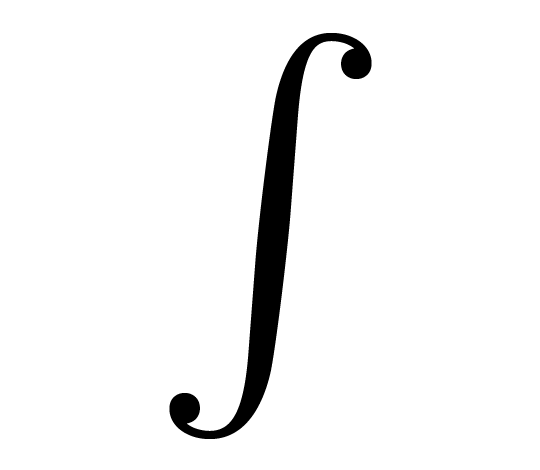
\includegraphics[width=1.0in]{img/logo.png},\centerline{a picture}]
% Duis aute irure dolor in reprehenderit in voluptate velit esse cillum dolore eu fugiat nulla pariatur. Excepteur sint occaecat cupidatat non proident, sunt in culpa qui officia deserunt mollit anim id est laborum
% \end{window}

%%%%%%%%%  Front matter   %%%%%%%%%
\begin{document}
\maketitle
\begin{minipage}[t]{.45\textwidth}\thispagestyle{empty}
  \vspace{-11mm}
  \tableofcontents
\end{minipage}% 
\begin{minipage}[t]{.1\textwidth}\thispagestyle{empty}
  \;
\end{minipage}% 
\begin{minipage}[t]{.45\textwidth}\thispagestyle{empty}
  \footnotesize
  \setlength{\parskip}{5pt}
  \vspace{-7mm}
  {\itshape
  Get ready for AMC 8 by participating our SIMC 8 in January, 2023!
    \begin{center}
        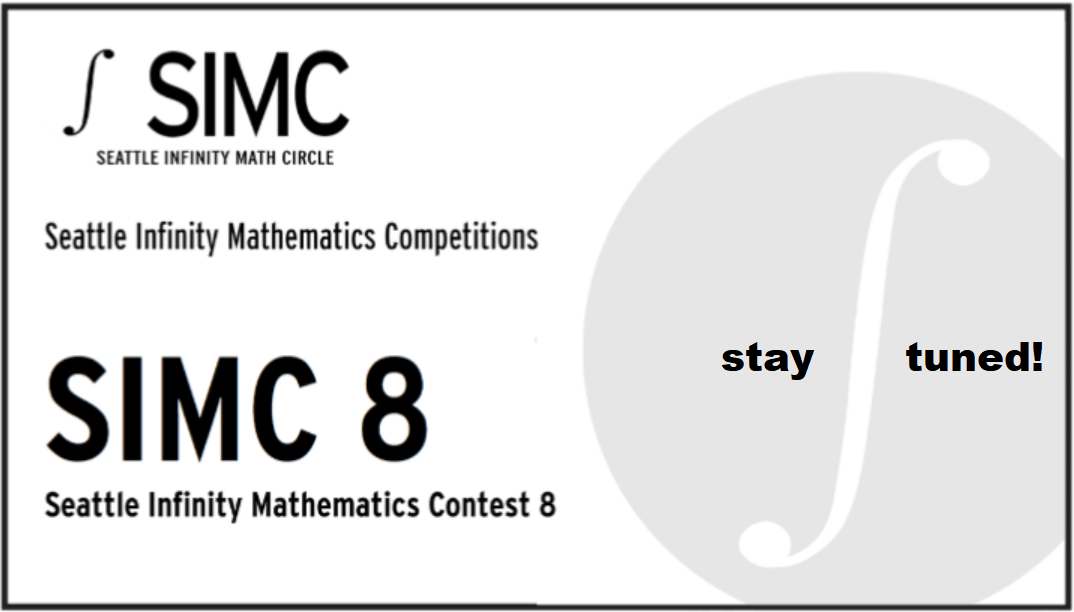
\includegraphics[scale=0.13]{Magazines/img/Vol3/simc8.png}
    \end{center}
}
\end{minipage}

\vspace{3mm}


\begin{multicols}{3}

\articletitle{Recursion Problems}{William Y. Feng}{}

Of all the techniques used to solve computational contest problems, recursion is undoubtedly my favorite. In this article, we'll explore a couple of recursion problems, and I'll share some ways I like to frame them.
\begin{center}
    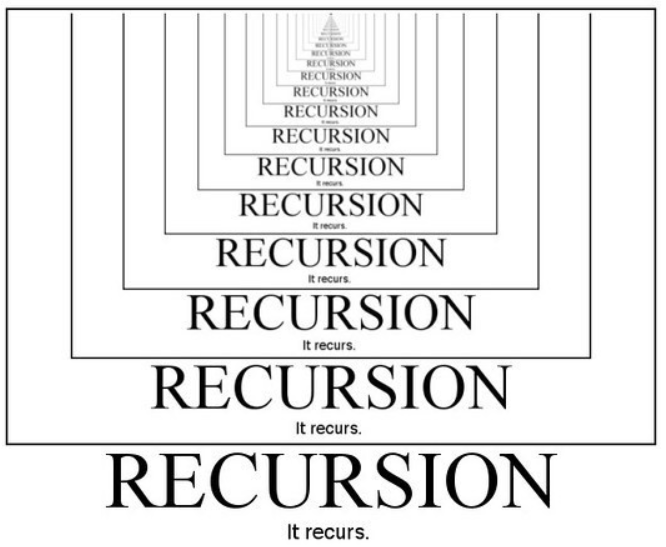
\includegraphics[scale=0.6]{Magazines/img/Vol3/recursion.png}
\end{center}
\textbf{Single-parameter recursion}
The simplest of recursions are those that rely on only one variable. Here's an example from the \textit{2007 AMC 12A}:

\textit{Call a set of integers spacy if it contains no more than one out of any three consecutive integers. How many subsets of $\{1,2,3,\ldots,12\},$ including the empty set, are spacy?}

At a high level, the formula for recursion problems is:
\begin{enumerate}
\item Find a \textit{function} and its associated \textit{parameters} that interest us.
\item Figure out the function in terms of itself evaluated at smaller parameters—this is known as the \textbf{recurrence relation} or \textbf{state transition}.
\item Evaluate the function at increasing parameters, starting at the \textit{base cases}, and working up to what we want.
\end{enumerate}
It's not always clear where to start finding a function. Do we want \texttt{spacy\_of\_size(n)}, a function that counts the number of spacy subsets with $n$ elements? Or perhaps we want \texttt{spacy\_with\_largest(n)}, a function that counts the number of spacy subsets whose largest element is $n$.

It takes experience finding the right function to use, and often times it's not at all intuitive. For this problem, we'll use \texttt{spacy\_max(n)}, a function that counts the number of spacy subsets of $\{1, 2, 3, \dots, n\}$. (The answer to the problem is this function evaluated at $n=12$.) For the sake of concision, let's rename this function to $f(n)$; then, we have the \textit{recurrence relation}
$$f(n) = f(n - 1) + f(n - 3).$$Why is this true? Let's imagine that we're constructing a spacy subset of $\{1, 2, 3, \dots, n\}$. What choices would we make? Well, we could either include or exclude $n$.
\begin{enumerate}
\item If we include $n$, then we can't include $n - 1$ or $n - 2$ due to the spaciness condition, but we can include any lower numbers—in other words, we can tack on any subset of $\{1, 2, 3, \dots, n - 3\}$, so long as it satisfies the spaciness condition. This is precisely $f(n - 3)$.
\item If we \textit{don't} include $n$, then we can do whatever we want with the remaining numbers—in other words, we can include any subset of $\{1, 2, 3, \dots, n - 1\}$ that itself satisfies the spaciness condition. This gives $f(n - 1)$ subsets.
\end{enumerate}
And with that, we have written $f(n)$ in terms of itself, evaluated at smaller parameters. We'll often find ourselves doing this sort of casework to break down the recurrence relation.

Now all that remains is a straightforward computation of $f(12)$. I like to start by evaluating $f(1), f(2)$, etc. and work my way up, keeping my previous computations \textit{cached} in a table. For instance, here's what the table would look like for while computing $f(6)$ (clipped):
\begin{table}[h!]
    \centering
    \begin{tabular}{c|c|c|c|c|c|c|c}
         $n$ & 1 & 2 & 3 & 4 & 5 & 6 & \dots \\\hline
         $f(n)$ & 2 & 3 & 4 & 6 & 9 & & \dots
    \end{tabular}
\end{table}
Computing $f(6)$ is then as simple as looking up the values of $f(5)$ and $f(3)$, and summing them. Completing the table gives $f(12) = 129$.

\textbf{Multi-parameter recursion}
Some problems utilize recursion with \textit{multiple} parameters. Here's an example from the \textit{2016 AIME II}:

\textit{The figure below shows a ring made of six small sections which you are to paint on a wall. You have four paint colors available and you will paint each of the six sections a solid color. Find the number of ways you can choose to paint the sections if no two adjacent sections can be painted with the same color.}
\begin{center}
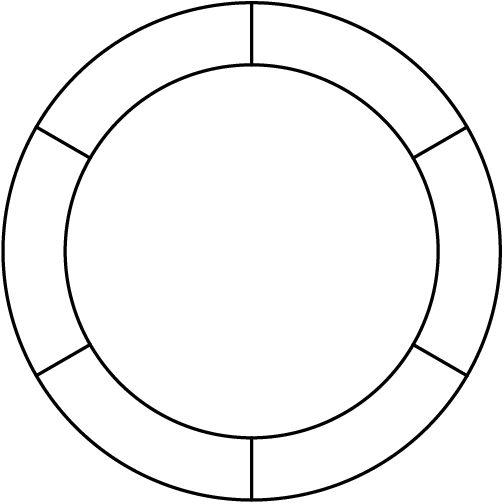
\includegraphics[scale=0.35]{Magazines/img/Vol3/2016_aime_ii_p12.png}
\end{center}

Let's first define the function:
\begin{enumerate}
    \item We want some function that depends on multiple parameters and counts the number of ways to paint \textit{something}.
    \item Now that we've gotten a taste of what recursion looks like, it seems natural that one parameter we should recurse on changes the \textit{size} of the problem. In this case, we'll let the parameter $n$ restrict ourselves to the first $n$ sections on the ring (starting, say, at the upper-right section).
    \item Paint colors are also a thing, so let's create another parameter, $k$, that determines what color of paint we must use in the last section painted. This is motivated because our choice of paint for a section depends on the paint used for the last section painted.
\end{enumerate}
We thus have a function, $f(n, k)$ that counts the number of ways to paint the first $n$ sections, where the last color must be color $k$. (We have numbered the paints 1, 2, 3, and 4.)

We have one minor complication, however. This is a \textit{ring}, so our choices of paint for the sixth section depend on the color of the first section. To deal with this, we exploit some symmetry—if we \textit{fix} the paint of the first section to be, without loss of generality, paint 1, then we know the last section must be painted with paints 2, 3, or 4. Thus, we impose one additional condition on $f$: now, $f(n, k)$ counts what it did before, but the first section must be color 1. Our answer will therefore be
$$4 \cdot (f(6, 2) + f(6, 3) + f(6, 4))$$
as we need to paint all 6 sections, but the last section cannot be color 1, and we multiply by 4 to account for the fact that we chose the first section to be color 1 arbitrarily.

What's our recurrence relation? Casework can help us here! To find $f(n, k)$, the number of ways to paint the first $n$ sections where the last section is color $k$ and the first section is color 1, consider that we have to have first painted the first $n - 1$ sections, and the last section cannot have been color $k$. Thus, we simply sum up the number of ways to paint $n - 1$ sections with the last section a color $i \neq k$:
$$f(n, k) = \sum_{i \neq k}^{n} f(n - 1, i).$$
We can use a table for this! Here's the table in the midst of evaluating $f(5, k)$:
\begin{center}
    %% Thanks, https://artofproblemsolving.com/wiki/index.php/2016_AIME_II_Problems/Problem_12
    \begin{tabular}{c|c|c|c|c }
        \multicolumn{1}{c}{}&\multicolumn{4}{c}{\(k\)}\\
        \(n\)&1 & 2 & 3& 4 \\ \hline
        1& 1 & 0 & 0 & 0\\
        2 & 0 & 1 & 1 & 1 \\
        3& 3 & 2 & 2 & 2 \\
        4 & 6 & 7 & 7 & 7 \\
        5 & & & & \\
        6& & & & \\
    \end{tabular}
\end{center}
To find $f(5, 1)$, for instance, we sum up the three 7s under $k=2, 3, 4$ in the previous row to get 21. To find $f(5, 2)$, we sum up $6 + 7 + 7 = 20$. Again, caching our computations in a table eliminates redundant computations.

A note about the base case for this problem: $f(1, 1) = 1$ while $f(1, 2) = f(1, 2) = f(1, 3) = 0$ because we specified that in all colorings that $f$ counts, the first segment must be color 1. Completing the table gives the answer of \textit{732}.

The exact same technique can be used on problem 16 from the 2011 AMC 12A:
\begin{quote}
    Each vertex of convex pentagon $ABCDE$ is to be assigned a color. There are $6$ colors to choose from, and the ends of each diagonal must have different colors. How many different colorings are possible?
\end{quote}
Try to use multi-parameter recursion to solve this problem!

\textbf{Conclusion} Approaching problems with recursion has given me a more methodical and robust problem-solving strategy; it's helped reduce casework and computation while increasing confidence in my answer.

In addition to contest math, recursion is an extremely useful concept in \textit{competitive programming} as well, in the form of \textit{dynamic programming}\footnote{\url{https://en.wikipedia.org/wiki/Dynamic\_programming}}. The scale of function parameters is much larger in programming problems, but the core principle of finding a function, figuring out its recurrence relation, and computing the answer.
\closearticle

\articletitle{On Learning Math}{Michael Yang}{}
I first learned about the area of a circle in second grade when our teacher gave it to us as a formula to use. Now, I should get one thing straight — even though I love all the beauty and ingenuity in math, I am, despite my best efforts, unfortunately not a naturally experimental mind. As a result, I was more than content to sit down and compute areas of different-sized circles without knowing why the formula was true. (Perhaps ironically, what I really took an interest in was the value of pi; this led to me memorizing many more digits of it than I will ever need.) 

In fourth grade, geometry struck again; I was introduced to the volumes of the cylinder, sphere, and cone. I vividly remember when our class measured three cones’ worth of water, then poured it all into a cylinder of the same radius and height. We were all so surprised when the volumes fit perfectly! Afterwards, many of my classmates crowded around our teacher, begging to know why it was true. Embarrassingly, I was again not one of them. “Ah,” I thought, “it’s obviously because we can somehow stack the three cones perfectly inside the cylinder! What could be more natural?” 
\begin{center}
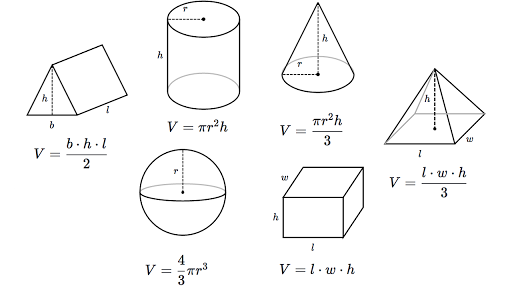
\includegraphics[scale=0.33]{Magazines/img/Vol3/geo_figures.png}
\end{center}
Unfortunately, I quickly learned that the answer wasn’t that simple. In middle school, I repeatedly heard that the volumes of these seemingly “easy” solids actually required something called integration, whatever that meant. And yet, I still wasn’t bothered enough to look anything up. In a repeat of my second-grade self, I was content to plug in numbers into math competition problems, pausing only to groan whenever I messed a formula up. 
\begin{center}
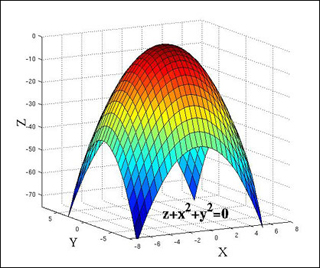
\includegraphics[scale=0.45]{Magazines/img/Vol3/multivar.jpg}
\end{center}
It was only a few months ago, when I was taking a multivariable calculus class, that I finally saw the machinery behind why these formulas are true. Our teacher presented us with a monstrous triple integral one day as a “warm-up problem” — making our dissatisfaction audibly known, our table slogged through the pages of computation. But what really surprised us was the answer: an integer multiple of pi. As it turns out, what we had actually done was to compute the volume of a cone in disguise! The cylinder and sphere quickly followed; just for fun, we did the circle, too. And thus, in that one hour, I resolved the questions which I hadn’t been willing to ponder for the past decade. 

What did I learn from all this? Well, be curious — if I had looked at the origins of these formulas earlier, I might have gotten interested in calculus and higher math long before I actually did. But I also think that there’s another point at play here: one of math history. There was a reason why we needed to appeal to triple integrals to determine the volume of a cone: the math we learn in second grade might be simple, but it’s definitely not easy. These sorts of problems stumped even the brightest minds of the Ancient Greeks; even though Archimedes almost certainly knew of these formulae, he famously lamented that he could not make his methods rigorous. It took until the late seventeenth century (almost two millennia later!) — when Newton and Leibniz introduced calculus — to make the proofs airtight. 

Math carries with it an incredible history, one that reverberates through time and space. It’s one that is truly international, with amazing math coming from every corner of the world. And, at its core, math is about collaboration. The proof of the area of a circle wasn’t found alone; neither was the volume of a sphere. The average high schooler now knows geometry unknown to Euclid and number theory unknown to Gauss not because our generation is that much better, but because we’ve been able to build off their work and the work of those that have come after them. 

Too often in the way math is first presented, the focus is on getting the answer right: you either use the formula correctly or you don’t. What too often goes unsaid is that some of the most brilliant mathematicians undoubtedly struggled proving the formula you’re using. And that’s why studying math history is so important: we can appreciate just how far we’ve come as a collective. 

So next time you encounter a formula you don’t know how to prove, ask yourself not just why, but also how, we know it’s true. Who knows? Sometime in the future, high school students may very well be solving the hardest open problems of our generation as warm-ups. 
\begin{center}
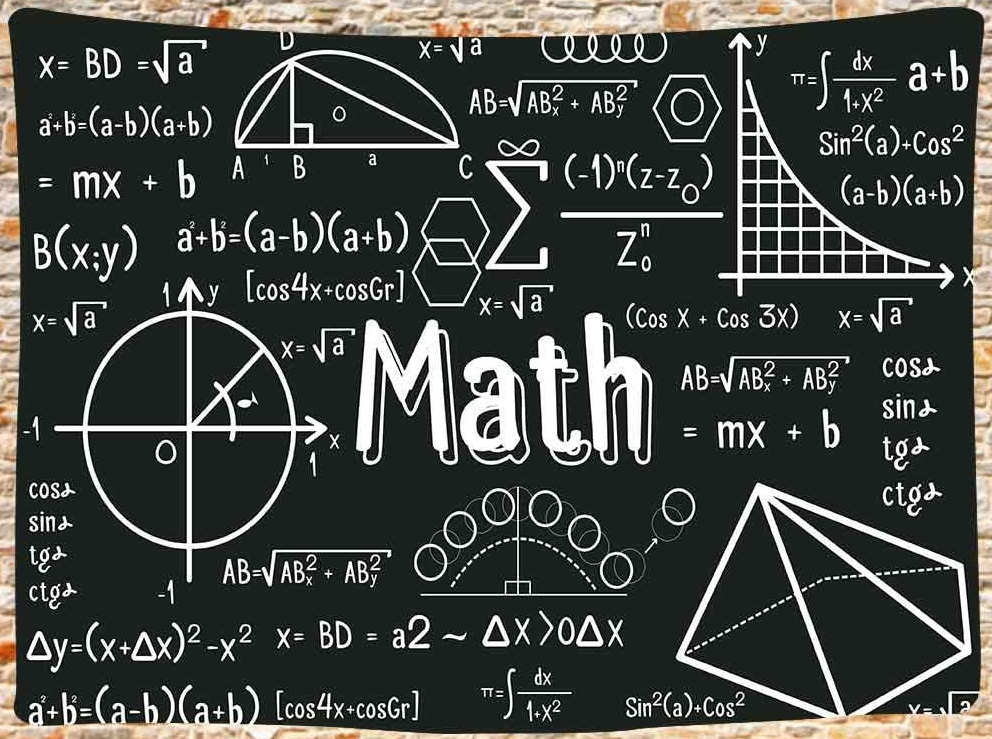
\includegraphics[scale=0.45]{Magazines/img/Vol3/math_p.png}
\end{center}
\closearticle

\end{multicols}

\articletitle{Probability}{Edward Yu}{}
\begin{center}
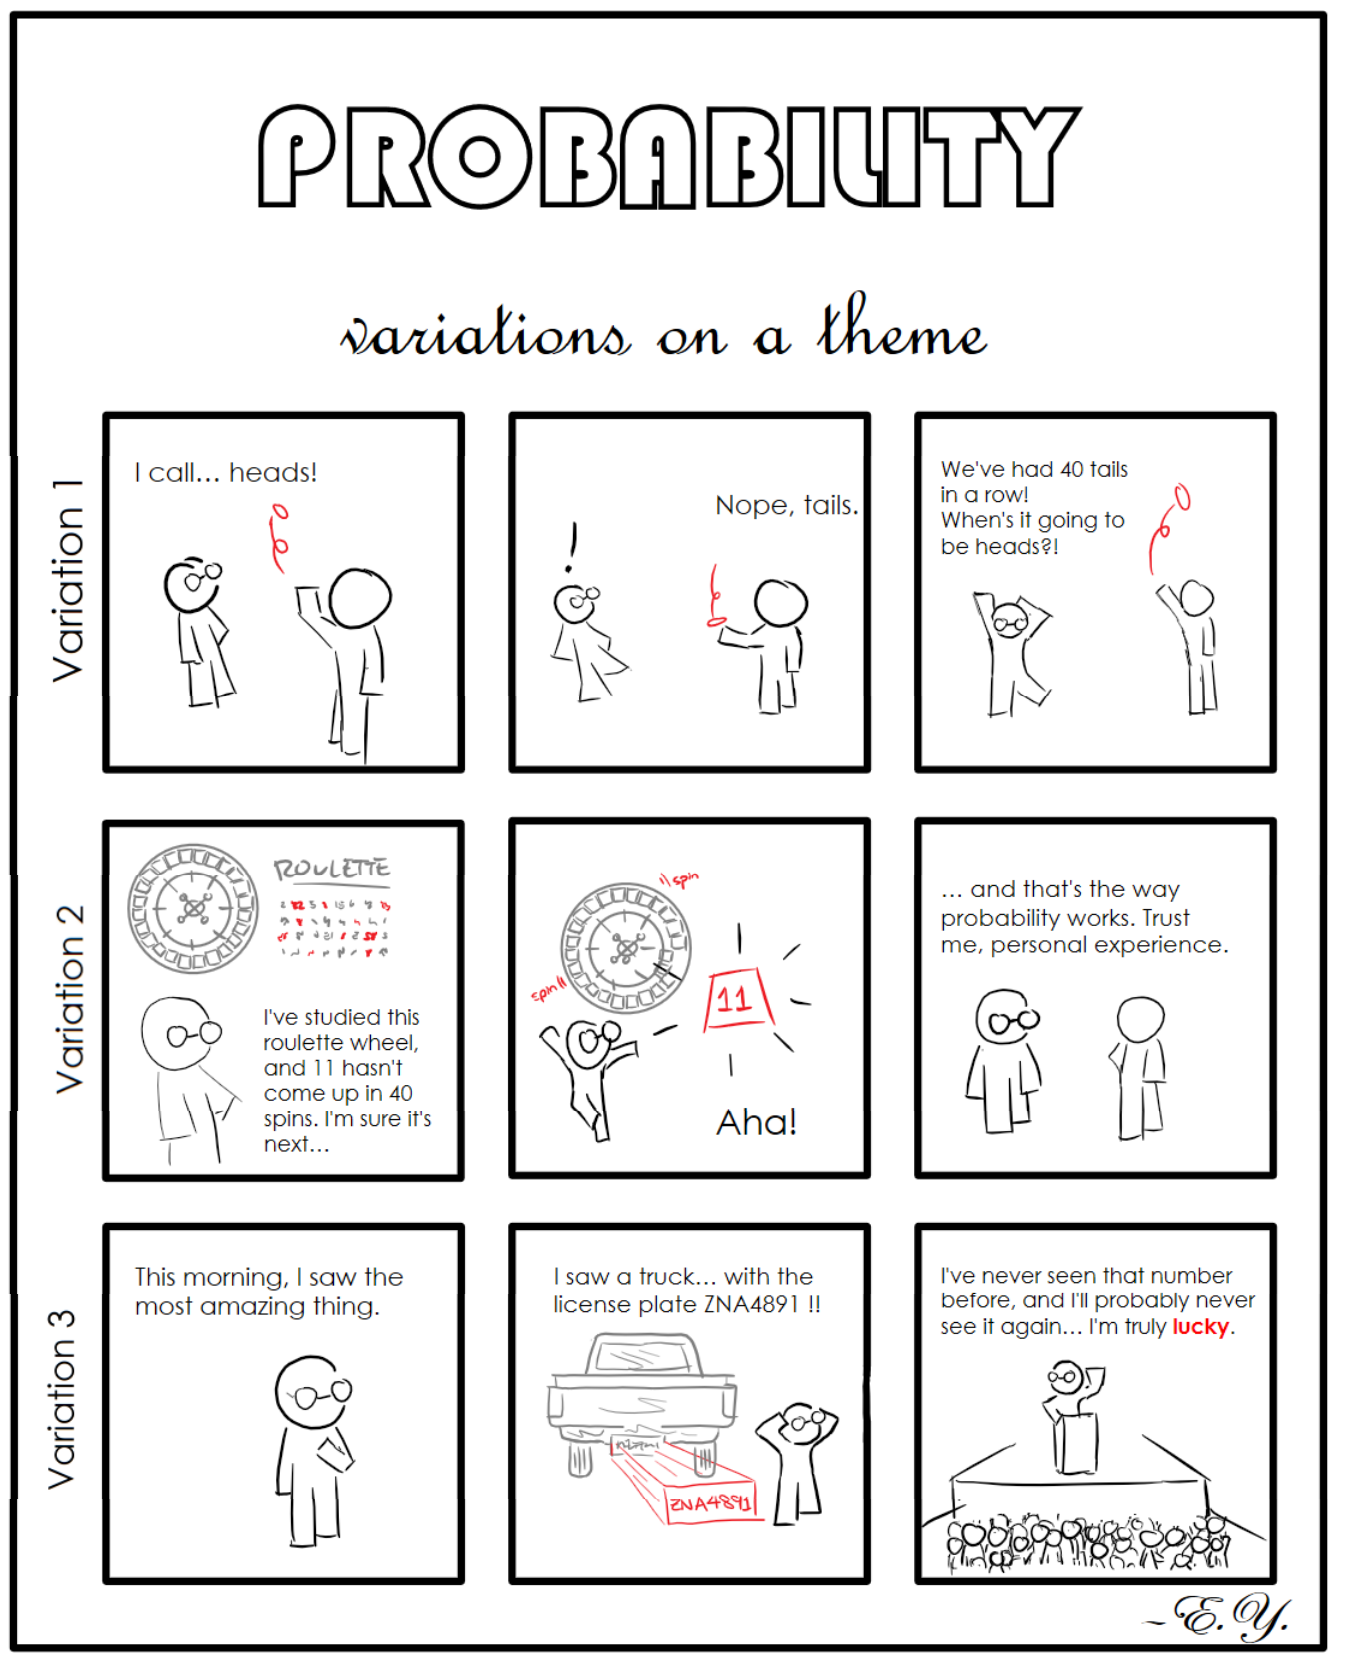
\includegraphics[scale=0.65]{Magazines/img/Vol3/probability.png}
\end{center}
\closearticle
\newpage
\begin{multicols}{3}

\articletitle{The Youtube Math Channels}{Michael Yang}{}
It's no secret that there is some great educational math content on the internet -- however, one area that often goes a bit overlooked is YouTube! Here are a few quick introductions to some of the main math YouTubers. 
\begin{center}

\includegraphics[scale=0.35]{Magazines/img/Vol3/youtube.2022.12.png}
\end{center}
The channel Numberphile, run by videographer Brady Haran, is perhaps the oldest well-known math channel still producing videos. Originally with videos focusing exclusively on one number and documenting several interesting facts about it, Numberphile has now broadened its scope to more general mathematical topics. For each video, Brady chooses a well-known mathematician to interview about a topic of their choice. Amazing math is then presented on Numberphile's classic brown paper, giving it a familial aura while also exploring some genuinely deep and fascinating topics. Additionally, videos are released quite frequently (often with just a few weeks between them!), and the interviewed mathematicians come from a variety of diverse cultures and backgrounds. Some highlights of Numberphile include Neil Sloane talking about incredible sequences, Hannah Fry on the mathematics of love, and Matt Parker with the Parker Square. Speaking of which... 
\begin{center}

\includegraphics[scale=0.35]{Magazines/img/Vol3/numberphile.png}
\end{center}
Of famed mathematical hilarity, the channel Stand-Up Maths is becoming more and more well-known. Run by mathematician Matt Parker, the channel aims to make math easy and fun to learn through the unlikely medium of stand-up comedy. In each video, Matt tackles what seems at first like a horribly difficult math problem with a mix of intriguing computer visuals, deep research papers, silly physical props, and his trademark enthusiasm. Known for "giving things a go," Matt is more than happy to post his (occasionally embarrassing!) attempts at tasks such as proving unsolved conjectures and measuring the radius of the Earth on the internet. What's never compromised, though, is the math(s): Matt is always sure to make his arguments airtight and is always willing to point out one of his past mistakes. 

Perhaps viewed as the gold standard of production quality, mathematician Grant Sanderson's channel 3blue1brown is a gold mine for eloquent explainers on some seriously intriguing math. Grant's education is no joke -- he graduated with a math degree from Stanford -- but his clear and intuitive explanation style has won over the hearts of many a math enthusiast. 
\begin{center}
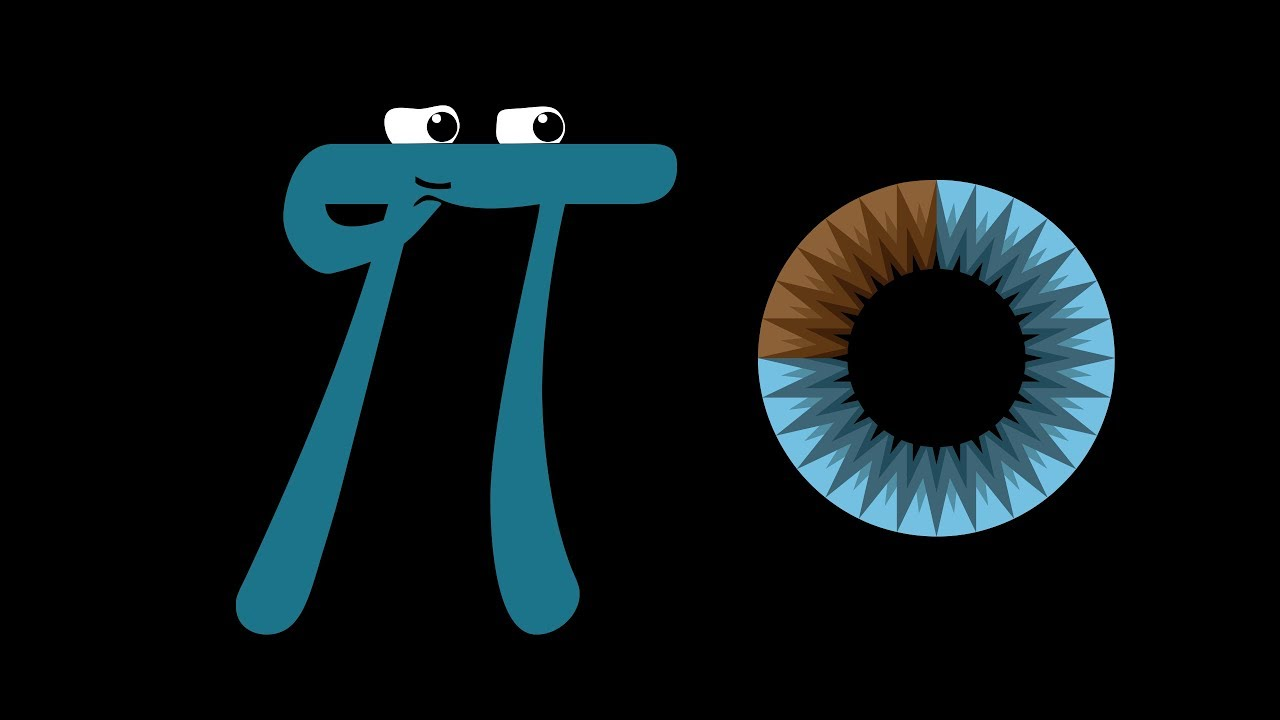
\includegraphics[scale=0.125]{Magazines/img/Vol3/3b1b.jpg}
\end{center}
With an emphasis on building intuition over rote computation, each 3blue1brown video strives to emphasize the visual beauty of mathematics. Perhaps unsurprisingly, the quality is top-notch: with fluid animations put together with meticulous care, Grant has cultivated a unique style and online presence. His video series on Calculus and Linear Algebra, in particular, have served as helpful building blocks for many future learners; his "Lockdown Math" livestreams, done in the middle of the pandemic for a high-school audience, has also garnered critical acclaim. 

Of course, there are many more excellent math-related YouTube channels out there (Vihart and Veritasium, anyone?) as well, and this is by no means an exhaustive list. And while YouTube is of course not an exhaustive math repository, it can be a useful resource for finding both quirky mathematical facts or deep proofs to some of the hardest theorems of our day. 
\closearticle

\articletitle{Cryptography}{Rohan Dhillon}{}
You have a message and you want to send it to a friend…but no one else can know about it. An age-old problem that has spurred a nuclear arms race to this day. Initially, the only way to achieve this was by walking, then horseback, then carrier pigeons, then the telegraph, then the telephone, and now, the internet. But someone can still “listen in” on the internet in the same way that someone can “guess” your password. How do they do it, and how do we protect ourselves?

The crux of modern cryptography relies upon this very important fact: big numbers are hard to factor. Take the number 3266999807178999181—I’m sure that if you saw that number on a math contest, your reaction would be “nope,” and even if you enlist a Java program to help you, it will still take a few minutes to get that the number only has two prime factors: 999999937 and 3267000013. 

So, why is this useful? Well, say we want to tell our agent to log into our Credit Suisse offshore account (obviously, we wouldn't want other people to know about this). We use a variation of “factoring numbers takes a long time” by using primitive roots modulo a prime p. An integer $g$ with $0<g<p$ is a primitive root if and only if $g^{p-1} \equiv 1 \pmod{p}$ and $g^k \not\equiv 1 \pmod{p}$ for all $0 < k < p-1$. 

\begin{center}

\includegraphics[scale=0.5]{Magazines/img/Vol3/crypto.png}
\end{center}

Both the agent and we decide to use the prime 11 as our modulo and $g=7$ as our primitive root. Both of these numbers are publicly available, but each of us has one number that is secret: we have $a=9$ and our agent has $b=4$. We can encrypt \textit{our} message by sending our agent $g^a \equiv 7^9 \equiv 8 \pmod{11},$ and our agent can send us $g^b \equiv 7^4 \equiv 3 \pmod{11}$ publicly. To decrypt the message, both of us take what we received to the power of our private key. We will get $3^9 \equiv 4 \pmod{11}$ and our agent will get $8^4 \equiv 4 \pmod{11},$ the same message! Intuitively, this makes sense as $g^{ba} \equiv g^{ab} \pmod{p}.$

Of course, this seems to not be \textit{that} useful since you both end up with a message, but this type of cryptography is usually used to set up a different, more efficient type called symmetric-key cryptography. As the name suggests, we both need the same key, but we don't want anyone else to know about it. And so both of us will start with two publicly known keys and then encrypt, exchange, and decrypt to get the same, now secret, key...now what?

We have the key 4, which is 100 in binary. Suppose we want to send the code 01101111 01110000 01100101 01101110, which corresponds to the word "open" using ASCII characters (each letter and typed symbol--not Unicode character--corresponds to a number between 0 and 128). In the simplest case, we can just use XOR encryption which returns a 1 if and only if the codes have different values at that position. Doing this yields a new code: 11111101 00111001 01000001 11111100, which we may send to our agent. They also have the key 100, and they can just apply the XOR function to the code they received to get the message: 01101111 01110000 01100101 01101110, "open."

And now our agent knows to open the offshore Credit Suisse account we've been storing our stock earnings in! Usually with this type of encryption and decryption, we would use \textit{giant} numbers with hundreds of digits to make sure that anyone trying to crack the code would have to wait until the death of the sun to do so. Interestingly, this is also why prime numbers are so important in our modern lives--there's even a book with random large primes that's on sale for \$60. After that not-at-all tax-evasionary article, I hope you walk away with a greater understanding of the real use mathematics has in our modern life--whenever you cry out "when will I ever use this in my life??" during math class, chances are you already have. 
\closearticle
\articletitle{The Story of 24 Point}{Owen Xuan}{}

Start with four cards, face up. Glance at their numbers: $7, 6, 12, 4$. The aim of the game is to manipulate these four numbers into equalling twenty-four, by using multiplication, division, addition, subtraction, and parenthesis. Aha! You find a solution:  $12 \times 6 / (7-4)$ equals twenty-four. Among other names, this card game is named 24 point. Standing on a deceptively straightforward foundation, 24 point is both malleable and lively. 

My first experience with 24 point came when I was 7, likely playing at our dinner table. We would split the deck into halves, then have each player flip two cards over and arrange them in a square. Thus ensued a state of full concentration: each round ended in either mutual shaking of heads and a redraw, or an excited table slap, which signaled a player had found a solution. Soon, I found myself bringing a deck of Bicycle playing cards on the bus, solving puzzles against an imaginary opponent. A distinctive quality of 24 point was that it could easily be played with a single person, and was portable, unlike solitaire. 

\begin{center}
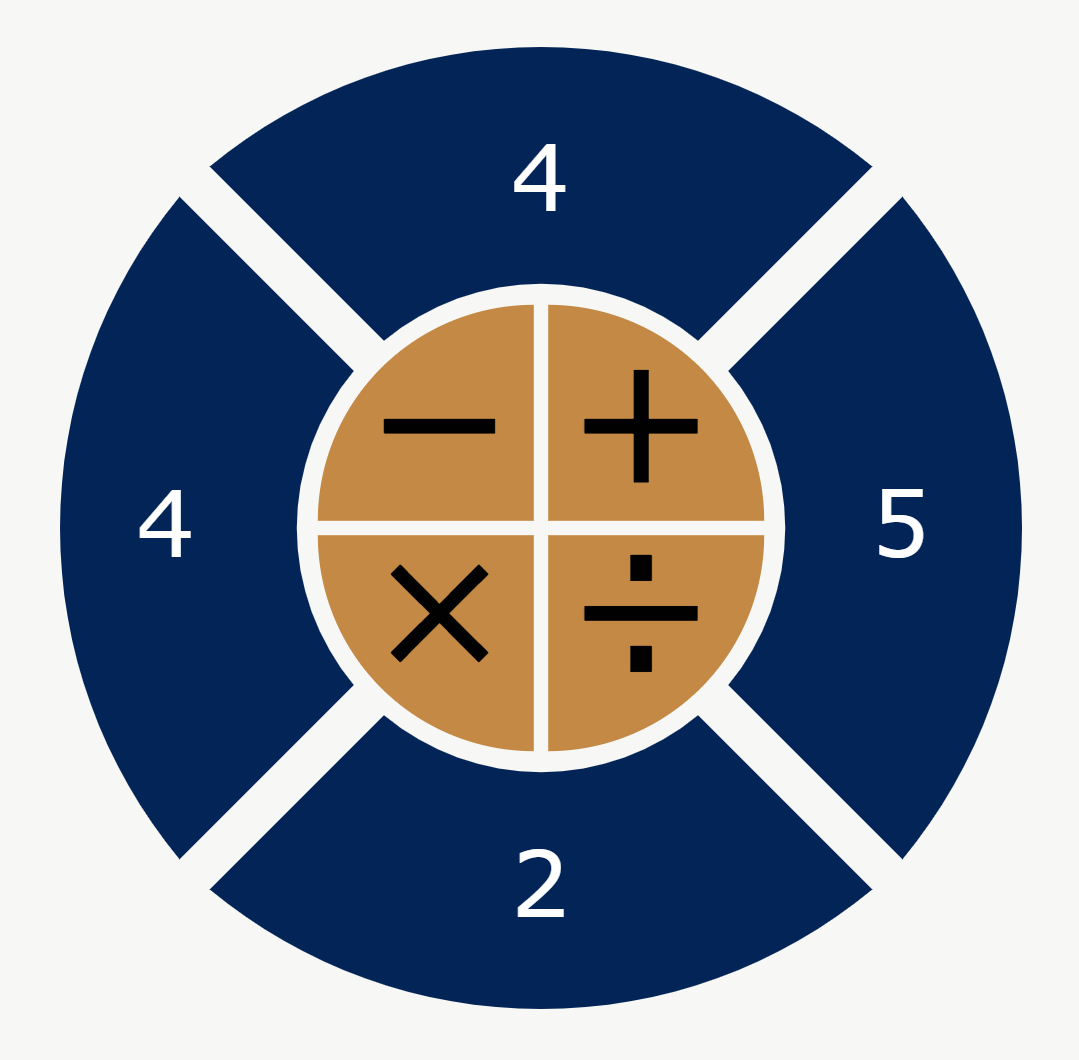
\includegraphics[scale=0.25]{Magazines/img/Vol3/24.png}
\end{center}

There’s a certain beauty to the complexity arising from the simple framework. Some arrangements of four cards are clear at a glance, whereas others, notably $[3 3 8 8]*$, look easy but require some thought. If we allow order and parenthesis to matter, even the combination $[1 2 3 4]$ has 194 solutions. Over time, certain puzzle-solving rules of thumb emerge. One quick technique is to build factors of 24, most commonly 3, 8 and 4, 6. Another strategy is to go a bit over 24, then subtract a card to return to the desired number, such as in the case $[3 3 3 3]$.

As one might expect, there are many arrangements of cards which are impossible to solve. With our current rules, $[1 1 1 1]$ is impossible (easy to verify), and so is $[3 3 5 11]$ (harder to verify). A full database of solvable and unsolvable combinations can be found here. Interestingly, around $25\%$ of combinations are unsolvable with our current available operators $(+ - * /)$ but if we introduce factorials, this number drops twenty-five fold to just below $1\%$. 

Perhaps the most valuable quality of the game is its adaptability. Since the main theme of the game is to create one number out of four, it can be modified without losing its nature. Frequently, players will allow new operators to boost the probability of getting a solvable set of cards, such as allowing exponentiation, square roots and logarithms. Factorials and permutations are also sometimes added, although some argue that it makes the game too easy (simply getting to 4, then using the factorial operator gets to 24). Other semi-common changes include changing the target number or changing the amount of cards used.

If we wish to venture beyond these standard variations, 24 point can be engineered to become more challenging, or cover concepts from more diverse fields of mathematics. To do this, we can increase the difficulty in two steps: removing “simple” operators and adding “complex” ones. Instead of using addition $(f(x,y) = x+y)$, what if we let $f(x,y) = 3x+y$? Or let an operator return the sum of the digits of the product of the two inputs? Or, going on a wild limb, creating an operator which takes in n cards, calculates the derivative of the polynomial $P(x) = x(\sum_{i=1}^n (a_i \cdot x^i))$, and returns the sum of the resulting coefficients? Once one starts tinkering with alterations, the flexibility of the game becomes obvious.

For educators, 24 point is an ideal game to both stimulate the brain and provide breaks from lectures. In addition to its flexibility, 24 point can provide a degree of competitive spirit (while still retaining some element of chance, for weaker students), or alternatively can be played in teams. The game is ripe with patterns, meaning players will likely feel a sense of progress as they begin to recognize more and more patterns within the random combinations of cards. Moreover, unlike the majority of “math games” within schools – even with discounting coolmathgames – 24 point builds arithmetic skills and critical thinking. In short, 24 point has the perfect build for a math game: short and sweet, helpful, flexible, satisfying. 
\closearticle

\articletitle{A Lanyard Problem: Generalizations}{Cecilia Sun}{}
In the last newsletter, we investigated the $1$ out of $n$ version of the lanyard puzzle: given a lanyard and $n$ pegs, can we wrap the lanyard around the pegs in a way such that removing any one peg will cause the lanyard to fall? We showed that yes, this is possible, and discovered a construction that contains approximately $2n^2$ moves. 

This might prompt us to change the question: what if we color our pegs, with two red pegs and one blue peg, and want to hang our lanyard in a way such that removing the blue peg causes the lanyard to fall, removing both red pegs causes the lanyard to fall, but removing just one red peg will leave the lanyard hanging? The answer turns out to be \textbf{yes}\footnote{by lecture theory}, and the solution is quite similar to what we discovered in the $1$ out of $n$ version! 

The idea is to define a \textbf{superpeg} $S$ which represents both the red pegs. Wrapping the lanyard clockwise around the superpeg corresponds with wrapping clockwise around the first peg, then clockwise around the second peg. It might be tempting to define a counterclockwise wrap around the superpeg to likewise correspond with wrapping counterclockwise around the first peg, then counterclockwise around the second peg, but this won’t work for our purposes! We want everything to cancel when we wrap the lanyard clockwise then counterclockwise around the superpeg, but this means we actually want to start from the back. So, we actually define a counterclockwise wrap around the superpeg to correspond with wrapping counterclockwise around the \textit{second} peg, then counterclockwise around the first peg\footnote{this looks suspiciously like how we construct inverses; in fact, it literally is just an inverse}. 

Then, if we let our two red pegs be pegs $1$ and $2$, then we can define our \textbf{superpeg moves} to be $s=x_1x_2$ and $s^{-1}=x_2^{-1}x_1^{-1}$. 

Then, we can just use our two peg solution on the superpeg $S$ and peg $3$, which gives us the configuration $sx_3s^{-1}x_3^{-1}$; we can then substitute our superpeg moves in, yielding us 
\[x_1x_2x_3x_2^{-1}x_1^{-1}x_3^{-1}.\]

We can still use this approach even when we have multiple superpegs: if we have $n$ arbitrary subsets of pegs, and we want the picture to fall if and only if all the pegs in at least one subset have been removed, then we can simply create the $n$ superpegs, as above, and then apply the $1$ out of $n$ peg solution on the superpegs. 

Right now, our construction is very inefficient. For instance, if we have two subsets $A$ and $B$ such that $A\subset B$, then we are guaranteed that removing all the pegs in $B$ will cause the lanyard to fall, since we already know that removing all the pegs in $A$ causes the lanyard to fall! However, if we construct our function as usual, we are still including the redundant superpeg $B$, which we could certainly just remove. 

It turns out that the answer to this optimization problem for any general case involves objects called \textbf{monotone boolean functions}, which are out of the scope of this article, but the idea is to scrap the subsets entirely and instead define a fall function $f_p(r_1,r_2,\dots,r_n)$ to output either $1$ (the lanyard falls) or $0$ (the lanyard remains hanging), where each $r_i$ is $1$ if the $i$th peg has been removed and $0$ if the $i$th peg is still there. We can then use logical circuits to solve the problem in complete generality! 

Through this framework, we deduce that the optimal solution for most such questions grow exponentially. However, the solutions to the special $k$ out of $n$ pegs cases (where the lanyard falls after any $k$ pegs are removed) have polynomial-length solutions!

If you’re interested in reading more, check out the paper \href{https://erikdemaine.org/papers/PictureHanging_FUN2012/paper.pdf}{here} to learn more! 
\closearticle

\articletitle{More on Complex Numbers!}{William Gvozdjak}{}
If you've been following \textit{The Circle} for some time, you may recall discussions of the complex numbers in past volumes (if you don't, I highly recommend checking out Volume 2!). In this article, we'll go further into depth on the complex numbers: why are they useful, and how can they be used to derive equations and solve problems?

First, we'll discuss a quick recap of what we already know. In \textit{Special Numbers in Euler's Identity}, we learned \textbf{Euler's Formula}, which gives us that $e^{i\theta}=\cos\theta+i\sin\theta$, where $e$ is a real constant (roughly $2.71828$), $i$ is $\sqrt{-1}$, and $\theta$ is an angle. When $\theta=0$, this gives us \textbf{Euler's Identity}, proclaimed as one of the most beautiful identities in all of mathematics: $e^{i\pi}+1=0$. And in \textit{Imaginarily Complex; Really Simple}, we learned some applications of the complex numbers, such as a combinatorics problem.

Let's turn out attention to a few equations that cause students many headaches in school: the trigonometric summation formulas. The two most common ones, for $\sin$ and $\cos$, are as follows:
\begin{align*}
    \sin(\alpha+\beta)&=\sin\alpha\cos\beta+\sin\beta\cos\alpha \\
    \cos(\alpha+\beta)&=\cos\alpha\cos\beta-\sin\alpha\sin\beta.
\end{align*}
The main question is: why are these equations so obscure, and how can we possibly remember them? Surprisingly, Euler's Formula gives as an answer to this question. Let's look at Euler's Formula with $\theta=\alpha+\beta$:
\[e^{i(\alpha+\beta)}=\cos(\alpha+\beta)+i\sin(\alpha+\beta).\]
Also, using simple exponent properties, we know that this is equal to $e^{i\alpha}e^{i\beta}$. We can now apply Euler's Formula to each of the individual parts:
\[e^{i\alpha}e^{i\beta}=(\cos\alpha+i\sin\alpha)(\cos\beta+i\sin\beta).\]
Expanding and keeping in mind that $i^2=-1$, we know that this is equal to
\begin{align*}
&\cos\alpha\cos\beta-\sin\alpha\sin\beta \\&+i(\sin\alpha\cos\beta+\sin\beta\cos\alpha).
\end{align*}
Therefore, we know that
\begin{align*}
&\cos(\alpha+\beta)+i\sin(\alpha+\beta) \\
&=\cos\alpha\cos\beta-\sin\alpha\sin\beta \\
&+i(\sin\alpha\cos\beta+\sin\beta\cos\alpha).
\end{align*}
But if we have two complex numbers that are equal, then their real components must be equal, and their imaginary components must be equal. Hence,
\begin{align*}
    \cos(\alpha+\beta)&=\cos\alpha\cos\beta-\sin\alpha\sin\beta \\
    \sin(\alpha+\beta)&=\sin\alpha\cos\beta+\sin\beta\cos\alpha,
\end{align*}
exactly as we wanted!

Euler's Formula can also be used to solve geometric problems. One extremely beautiful application is 2020 AIME I Problem 8:

``A bug walks all day and sleeps all night. On the first day, it starts at point $O$, faces east, and walks a distance of $5$ units due east. Each night the bug rotates $60^\circ$ counterclockwise. Each day it walks in this new direction half as far as it walked the previous day. The bug gets arbitrarily close to the point $P$. Then $OP^2=\tfrac{m}{n}$, where $m$ and $n$ are relatively prime positive integers. Find $m+n$.''

At first, this problem seems very difficult: one could try out the first few days and look for a pattern, but a pattern is not obvious to see. Instead, we use complex numbers.

The first important thing to realize is that a complex number is a vector. Therefore, if we add two complex numbers, we are adding the vectors that correspond to those numbers. For example, the complex number $i$ added to the complex number $1$ gives their vector sum: $1+i$.

\begin{center}
    \begin{asy}
        unitsize(2cm);
    
        draw((0, 0)--(1, 0), EndArrow);
        draw((1, 0)--(1, 1), EndArrow);
        draw((0, 0)--(1, 1), red, EndArrow);

        label("$1$", (0.5, 0), dir(270));
        label("$i$", (1, 0.5), dir(0));
        label("$1+i$", (0.5, 0.5), dir(135));
    \end{asy}
\end{center}

Keeping this in mind, we can try and represent each day as a separate complex number. Then, summing all of these complex numbers will give us the point that the bug approaches.

Now, how do we find the complex number for each day? If we look close at Euler's Formula, we can see that the complex number $ae^{i\theta}$ is the vector starting from the origin and ending at the point $a$ away from the origin and $\theta$ counterclockwise from the $x$-axis:

\begin{center}
    \begin{asy}
        unitsize(1.25cm);

        draw((-1.5, 0)--(1.5, 0), EndArrow);
        draw((0, -1.5)--(0, 1.5), EndArrow);

        draw((0, 0)--1.25*dir(60), EndArrow);
        label("$2e^{i60^\circ}$", 1.25*dir(60), dir(15));
    \end{asy}
\end{center}

Therefore, the first day can be represented as the complex number $5e^{i0^\circ}$: it walks east ($0^\circ$ counterclockwise from the $x$-axis) for $5$ units (it walks to a distance of $5$ from the origin). Then, the next day, the bug turns $60^\circ$ counterclockwise and walks half the distance of the first day, giving us the complex number $\frac{5}{2}e^{i60^\circ}$. The same thing occurs the day after that, giving us $\frac{5}{2^2}e^{i(60\cdot2)^\circ}$. Continuing this and summing all of the resulting complex numbers gives us a final series of
\[5e^{i0^\circ}+\frac{5}{2}e^{i60^\circ}+\frac{5}{2^2}e^{i(60\cdot2)^\circ}+\dots.\]
But this is just an infinite geometric series with first term $5e^{i0^\circ}$ and common ratio $\frac{1}{2}e^{i60^\circ}$! Therefore, we can use the formula for the sum of an infinite geometric series $\frac{a}{1-r}$. Using this formula and Euler's Formula to simplify gives us a final position of
\begin{align*}
\frac{5e^{i0^\circ}}{1-\frac{1}{2}e^{i60^\circ}}&=\frac{5}{1-\frac{1}{2}\left(\frac{1}{2}+i\frac{\sqrt{3}}{2}\right)} \\
&=\frac{20}{3-i\sqrt{3}} \\
&=5+\frac{5\sqrt{3}}{3}i.
\end{align*}
Now, we're looking for the square of the distance between this point and the origin, so we want the squared magnitude of the above complex number. This is just
\[5^2+\left(\frac{5\sqrt{3}}{3}\right)^2=25+\frac{25}{3}=\frac{100}{3}.\]
This gives us a final answer of $100+3=\boxed{103}$.

In conclusion, Euler's Formula and complex numbers, when applied in the right context, can be used to greatly simplify computations and strategies. The next time you're working with trigonometric expressions or confusing geometry problems, try complex numbers!
\closearticle

\end{multicols}

\clearpage
\begin{center}
\vspace{1.5cm}
    
\includegraphics[scale=0.8]{Magazines/img/Vol3/call4submission.jpg}
\end{center}

\vspace{1.5cm}

\begin{center}
\sc\Large{\textbf{Contact Us}}
\begin{tabular}{c l}
  
\includegraphics[scale=0.06,valign=c]{Magazines/img/email.png}
    & \href{mailto:seattleinfinitymathcircle@gmail.com}{Email}\\
  \;\\
  
\includegraphics[scale=0.1,valign=c]{Magazines/img/website.png}
    & \href{https://seattleinfinity.org}{Website} \\
  
\includegraphics[scale=0.5,valign=c]{Magazines/img/facebook.png}
    & \href{https://www.facebook.com/simathcircle/}{Facebook} \\
  
\includegraphics[scale=0.5,valign=c]{Magazines/img/insta.png}
    & \href{https://www.instagram.com/seattleinfinitymathcircle/}{Instagram} \\
  
\includegraphics[scale=0.5,valign=c]{Magazines/img/youtube.png}
    & \href{https://www.youtube.com/channel/UCgwA-iysWPc_XG0R0AZ5z5g/videos}{YouTube} \\
  
\includegraphics[scale=0.013,valign=c]{Magazines/img/discord.png}
    & \href{https://discord.gg/2Ma3dURhTt}{Discord} 
\end{tabular}
end{center} 

\end{document}
